\documentclass[12pt]{book}
\usepackage{amsmath}
\usepackage{float}
\usepackage[margin=1.5in]{geometry}
\usepackage{enumitem}
\usepackage{xcolor}
\usepackage{cancel}
\usepackage{graphicx}



\title{Introduction to Mechanics}
\author{Nathan Butcher}

\begin{document}
\graphicspath{{Figures/Units}}
\newcounter{chp}
\setcounter{chp}{0}
\newcounter{example}

\newcommand{\scinot}[2]{#1 \cdot 10^{#2}}

%Start a new example using counters
\newcommand{\example}{\textbf{Example \texttt{\thechp}.\texttt{\theexample}}
\addtocounter{example}{1}

\hspace{10pt}}

%Give a horizontal line with space to separte things
%like examples or asides
\newcommand{\linespace}{\hspace{10pt}

\hrule

\hspace{10pt}}

\chapter{Introduction, Numbers, and Units}

\setcounter{example}{1}
\addtocounter{chp}{1}

In physics we study the interactions and motion of matter. For our introduction in this class, we will mostly study what I like to call ``Physics at the human scale'' because it is the physics of daily life that we observe and directly interact with. It describes an apple falling from a tree, a car slamming its brakes, a pendulum swinging, the collision of 2 billiard balls, and more.

\section{Math and scientific notation}

This text will assume that you are comfortable with using algebra to solve an equation for a variable and that you have had a class on trigonometry. We will review those topics as they come up but it may be difficult to follow without the math background.

During this text we will use \textbf{scientific notation} frequently to write very large or very small numbers in an easier to read format. With it, we write a number in the format

\begin{equation}
\scinot{a}{b}
\end{equation}

where $1 \leq a < 10$ and $b$ is an integer. This saves us from having to write and count a lot of zeros that indicate place. The number is a factor multiplied by a power of 10.

\linespace

\example

Write the number 38,500,000 in scientific notation.

\hspace{10pt}

To write this in the form $\scinot{a}{b}$, first let's find $a$ such that $1 \leq a < 10$. Since our number starts with the digits 385, that means $a = 3.85$. From here we have

\begin{equation}
38,500,000 = 3.85 \cdot 10,000,000
\end{equation}

Now we need to write 10,000,000 as a power of 10. There are 7 zeros, so it will be $10^7$. This means that our number is 

\begin{equation}
\scinot{3.85}{7}
\end{equation}

\linespace

\example

Write the number 0.000007018 in scientific notation.

\hspace{10pt}

We can use the same reasoning as the above example to find that $a = 7.018$. The number can be written as

\begin{equation}
0.000007018 = 7.018 \cdot 0.000001
\end{equation}

Now we just need to find the power of 10. Let's start looking at powers of 10.

\begin{equation}
\begin{split}
10^0 = 1 \\
10^{-1} = \frac{1}{10} = 0.1 \\
10^{-2} = \frac{1}{10^2} = 0.01 \\
10^{-3} = \frac{1}{10^3} = 0.001
\end{split}
\end{equation}

A negative power means to take 1 divided by the number to that positive power. Looking at 10, we see that as we decrease the power (larger negative value), we move the decimal point 1 to the left. This will give us

\begin{equation}
0.000001 = \frac{1}{10^6} = 10^{-6}
\end{equation}

which makes our number

\begin{equation}
0.000007018 = \scinot{7.018}{-6}
\end{equation}

\section{Units}

Physicists will try to describe the world around us quantitatively, meaning with numbers. In order to ascribe meaning to those numbers we need to use physical \textbf{units}. For example, think about if you were baking a loaf of bread and the recipe called for ``4 flour''. Would you know how much flour was required? The recipe should say ``4 \textit{cups} of flour'' so that you know the amount required for the bread. 

In physics, like most sciences, we use \textbf{SI units}. In the USA, you likely encounter the Imperial system of units in daily life. Common Imperial units you might have seen include the inch for length and gallon for volume. These units are not the standard for scientific disciplines, and as such we will focus on using SI units. There are 3 base units that we will use frequently:

\begin{itemize}
\item \textbf{kilogram} - the SI base unit of mass. Mass is a measure of how much matter there is. It is related to but not the same as weight. We will discuss weight further in a later chapter, but for now think of mass as how much ``stuff'' there is.

\item \textbf{meter} - the SI base unit of length. If you don't have a good mental picture of a meter, it is a little longer than 3 feet.

\item \textbf{second} - the SI base unit of time. We will continue to see minutes and hours used throughout, but for doing quantitative work we will want to use seconds for everything.
\end{itemize}

\section{SI Prefixes}

With these SI base units we use \textbf{prefixes} to scale the units relative to our problem. Table \ref{SIPrefixes} contains several of the most common prefixes, with the bolded ones being most important for this class.

\begin{table}[b]
\centering
\caption{SI Prefixes}
\begin{tabular}{ c | c | c }
	\hline
	Prefix & Abbreviation & Numerical value \\
	\hline
	nano- & n & $10^{-9}$ \\
	micro- & $\mu$ (Greek letter \textit{mu}) & $10^{-6}$ \\
	\textbf{milli-} & m & $10^{-3}$ \\
	\textbf{centi-} & c & $10^{-2}$ \\
	\textbf{kilo-} & k & $10^3$ \\
	mega- & M & $10^6$ \\
	giga- & G & $10^9$ \\
	\hline
\end{tabular}

\label{SIPrefixes}
\end{table}

One thing you should see is that SI prefixes allow us to scale our units by powers of 10. This is much simpler than the Imperial system. For lengths we have 12 inches to a foot, 3 feet to a yard, and 1760 yards to a mile. Compare this to just multiplying or dividing by powers of 10 and see how much simpler SI units are to work with!

The main purpose to having the prefixes is it allows us to scale the units to our problem. If we were to talk about the distance between San Diego and Los Angeles, it would make sense to use kilometers because that distance is about 194 kilometers. In meters, it would be $194 \cdot 10^3 = 194,000$ meters. Prefixes allow us to use numbers that are closer to 1, which are easier to read and for our brains to process. 

There are other prefixes and units that are used within different branches of physics and other fields of science. We will see some of this in CHAPTER HERE when we discuss the solar system. Again, the goal is always to make the numbers we work with closer to 1.

In addition to the base units, we will also have \textbf{derived units}, which are a combination of SI base units. On a car speedometer you may have seen the unit $km/hr$, which means ``kilometers per hour''. This is a derived unit because it combines the units of length and time.


\section{Converting units}

Now that we have SI prefixes, it is important that we learn how to convert between different units. This process is called \textbf{dimensional analysis} because the units are the ``dimensions'' that we are looking at.

To convert units, we will write unit factors that are fractions equal to 1. For example, 

\begin{equation}
\frac{1 \, mm}{10^{-3} \, m} = 1
\end{equation}

is a unit factor that equals 1 because the prefix milli- means $10^{-3}$, so 1 millimeter is equal to $10^{-3}$ meter. This fraction can by multiplied by a quantity to change the unit but not the physical value because the fraction is 1. Now lets use that to convert 3.25 meters to millimeters. We can use the unit fraction to cancel the meters from the original value, and have a unit of millimeters left in the numerator.

\begin{equation}
3.25 \, \cancel{m} \cdot \frac{1 \, mm}{10^{-3} \, \cancel{m}} = 3,250 \, mm
\end{equation}


The reason this works is that our unit fraction is equal to 1, so multiplying our original quantity by that unit fraction doesn't change the value! It only changes what unit that value is given in.

You could also think of the unit fraction as 1,000 millimeters in a meter.

\begin{equation}
3.25 \, \cancel{m} \cdot \frac{1000 \, mm}{1 \, \cancel{m}} = 3,250 \, mm
\end{equation}

Both $\frac{1000 \, mm}{1 \, m}$ and $\frac{1 \, mm}{10^{-3} \, m}$ are valid unit fractions for converting from meters to millieters. They are equally correct, so use whichever you prefer!

\linespace

%\textbf{Example \texttt{\thechp}.\texttt{\theexample}}
%\addtocounter{example}{1}
\example

\textbf{Convert 500 nanometers to centimeters.}

\hspace{10pt}

We can convert 500 nanometers to meters first, then convert from meters to centimeters.

\begin{equation}
500 \, \cancel{nm} \cdot = \frac{10^{-9} \, m}{1 \, \cancel{nm}} = 5 \cdot 10^{-7} \, m
\end{equation}

\begin{equation}
\scinot{5}{-7} \, \cancel{m} = \frac{100 \, cm}{1 \, \cancel{m}} = \scinot{5}{-5} \, cm 
\end{equation}

Sometimes it is useful to convert to an intermediary unit to help you get to the requested final unit.

\linespace

\example

Convert 1 meter to feet. Use the following information:

\begin{itemize}
\item 1 foot = 12 inches
\item 1 inch = 2.54 cm
\end{itemize}

The given unit conversions tell us how to solve this problem. First we convert the meter to centimeters, then use the given conversion from centimeters to inches. Finally, we can use the given conversion from inches to feet.

\begin{equation}
1 \, \cancel{m} \cdot \frac{100 \, \cancel{cm}}{1 \, \cancel{m}} \cdot \frac{1 \, \cancel{in}}{2.54 \, \cancel{cm}} \cdot \frac{1 \, foot}{12 \, \cancel{in}} = 3.28 \, feet
\end{equation}

\linespace

\example

A car is driving at 45 kilometers per hour $\frac{km}{hr}$. Convert this to meters per second $\frac{m}{s}$

\hspace{10pt}

First let's write out the unit to help us see how to convert this.

\begin{equation}
45 \, \frac{km}{hr}
\end{equation}

This means that the car moves 45 kilometers in 1 hour. When doing unit conversions it may be helpful to write out the unit like that

\begin{equation}
45 \, \frac{km}{hr} = \frac{45 \, km}{1 \, hr}
\end{equation}

We have kilometers in the numerator and hours in the denominator, so we have to make sure we write our unit fractions correctly to cancel them. First, let's convert the kilometers to meters.

\begin{equation}
\frac{45 \, \cancel{km}}{1 \, hr} \cdot \frac{10^3 \, m}{1 \, \cancel{km}} = \frac{45,000 \, m}{1 \, hr}
\end{equation}

Now we can convert the hour to seconds. It may be helpful to convert to minutes first, then to seconds.

\begin{equation}
\frac{45,000 \, m}{1 \, \cancel{hr}} \cdot \frac{1 \, \cancel{hr}}{60 \, \cancel{min}} \cdot \frac{1 \, \cancel{min}}{60 \, s} = \frac{12.5 \, m}{1 \, s}
\end{equation}

The car is driving at $12.5 \, \frac{m}{s}$.



\chapter{Quantities of motion and kinematics}
\setcounter{example}{1}
\addtocounter{chp}{1}

The first thing we must do to describe the motion of objects is define specific terms that we will use. These terms will have clear, specific definitions that may differ from how they are used in everyday language. 

\section{Motion definitions}

The first quantity to talk about is \textbf{position}. This is a measurement of where something is along an axis (or multiple axes). This is a length, so the SI unit for position is the meter. Position will be denoted with the variable $x$ in equations.

When we study motion, we often look at an object moving from one position to the other. The first position is the \textbf{initial} position, and the second position is the \textbf{final} position. In equations we will use subscript $i$ and $f$ for initial final respectively, so that the initial position is $x_i$ and the final position is $x_f$. To indicate the change in a quantity we will use $\Delta$, which is the Greek letter Delta. The change in position between the initial state and final state can be written as

\begin{equation}
\Delta x = x_f - x_i
\end{equation}

which is a measure of how the position changed moving from the initial state $x_i$ to the final state $x_f$. 

The second quantity we will talk about is \textbf{velocity}. This is a measurement of the rate of change in position of a moving object.  Velocity will be denoted with the variable $v$ in equations. Velocity has a direction, so it is a vector quantity. The direction can be denoted with a positive or negative sign to indicate the direction along a position axis.

\textbf{Average velocity} is the average rate of change in position as an object moves from its initial position $x_i$ to its final position $x_f$ over a time interval $\Delta t$. For average velocity we will use a subscript ``avg'', so it is written as $v_{avg}$. 

\begin{equation}
v_{avg} = \frac{\Delta x}{\Delta t}
\end{equation}

Average velocity does not give us any information about the moment-to-moment velocity throughout the motion, only the average throughout the time interval.

From the equation above, we see that velocity is a length divided by time. This means our SI unit is $\frac{m}{s}$ , which is read as \textit{meters per second}. 

The third quantity we will talk about is \textbf{acceleration}. This is a measurement of the rate of change of velocity of a moving object. Acceleration will be denoted with the variable $a$ in equations. Acceleration has a direction, so it is a vector quantity. 

\textbf{Average acceleration} is the average rate of change in velocity as an object moves from its initial position $x_i$ to its final position $x_f$ over a time interval $\Delta t$. Similar to position, the initial velocity is $v_i$, the final velocity is $v_f$, and the change in velocity is $\Delta v = v_f - v_i$.

\begin{equation}
a_{avg} = \frac{\Delta v}{\Delta t}
\end{equation}

Again, average acceleration gives us the average value over the entire interval of motion but no information about the moment-to-moment value of the acceleration.

From the equation above, we see that acceleration is a velocity divided by time. Our SI unit is $\frac{m/s}{s}$, which is read as \textit{meters per second per second}. The unit can also be written as $\frac{m}{s^2}$, which is read as \textit{meters per second squared}. These two ways of writing the units of acceleration are equivalent and both are correct. For the rest of this text, I will use $\frac{m}{s^2}$.

The final quantity we will introduce is \textbf{speed}. This is a measurement of how fast an object is moving. You might be familiar with miles per hour (mph) or kilometers per hour ($\frac{km}{hr}$) from a car speedometer. The SI unit of speed is $\frac{m}{s}$, same as velocity. Speed will be denoted as $s$ in equations.

\textbf{Average speed} can be found by taking the distance traveled $d$ over the time duration $\Delta t$.

\begin{equation}
s_{avg} = \frac{d}{\Delta t}
\end{equation}

One important issue we must address is how average speed differs from average velocity. Both are measured in units of $\frac{m}{s}$ and can be used to get information about how fast an object moved.

\begin{enumerate}
\item Speed is a scalar quantity, not a vector quantity. Speed does not tell you anything about the direction of motion. There is no such thing as a negative speed because the distance traveled will always be zero or positive.

\item The distance traveled is not always the same as the change in position. Velocity only depends on $x_i$, $x_f$, and $\Delta t$ with no concern for the path taken between $x_i$ and $x_f$. Speed depends on the distance traveled so it does matter what the path taken is.
\end{enumerate}

The last new definitions we will introduce here are \textbf{instantaneous speed} and \textbf{instantaneous velocity}. Instantaneous speed is a measure of the speed at an instant in time. Instantaneous velocity is the rate of change in position at an instant in time, which can also be thought of as the instantaneous speed plus the direction of travel.

\section{Motion Graphs}

One helpful tool for studying the motion of objects is to use graphs. This allows us to present data in a visual format rather than text. The x-axis will be the time and the y-axis will be position, velocity, or acceleration.

First, let's start with the following graph of position vs. time (which is also called an \textit{x vs t} plot).

\begin{figure}[H]
\centering
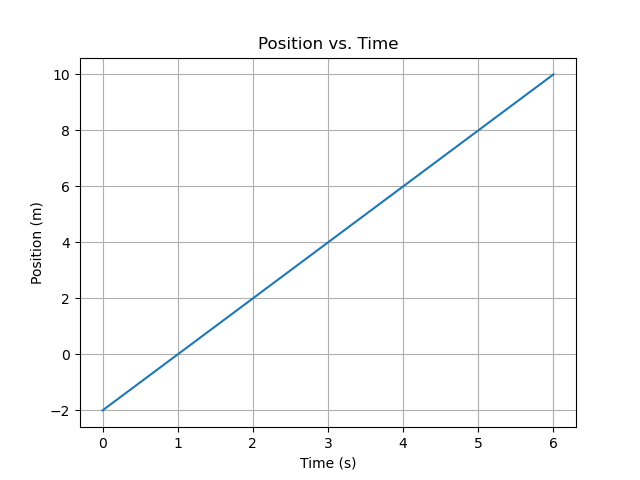
\includegraphics[scale=0.6]{position1.png}
\caption{Sample position vs. time graph}
\label{pos1}
\end{figure}

The graph has a title that tells you what the graph shows and the x- and y-axes are labeled, including units. These features are important to allow somebody reading your graph to easily understand what it is showing. 

This graph has time in seconds on the x-axis and position in meters on the y-axis. What this graph is showing is therefore the position of an object as it moves over time. For example, if we wanted to find the position of the object at $t = 4 \, s$ we would look at the y-value of the graph at $4 \, s$. The position of the object is therefore $x = 6 \, m$.

What if we wanted to find the average velocity of the object throughout this motion? It moves for 6 seconds, so $\Delta t = 6 \, s$. The position at $t = 0 \, s$ is $x = -2 \, m$, so we have in the initial state $x_i = -2 \, m$. The position at $t = 6 \, s$ is $x = 10 \, m$, so we have in the final state $x_f = 10 \, m$.

\begin{equation}
v_{avg} = \frac{\Delta x}{\Delta t} = \frac{10 \, m - (-2) \, m}{6 \, s} = 2 \, \frac{m}{s}
\end{equation}

Since our y-value is position and x-value is time, what we just did above is find the slope of the line! We can extend this in general to recognize that \textbf{the slope of a \textit{x vs t} graph is the velocity.} We can use this to find instantaneous velocities by finding the slope at a point on the graph! Below is a plot of velocity vs. time that describes the same motion.

\begin{figure}[H]
\centering
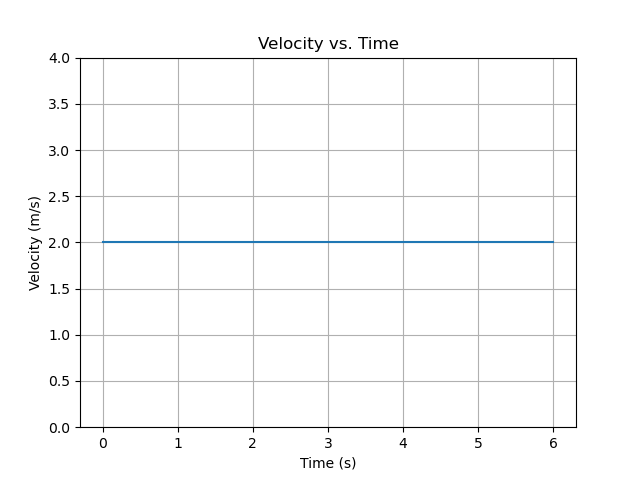
\includegraphics[scale=0.6]{velocity1.png}
\caption{Sample velocity vs. time graph for the same motion as \ref{pos1}.}
\end{figure}

The slope of the \textit{x vs t} plot is constant, so the velocity doesn't change throughout the motion. From $0 \, s$ to $6 \, s$ we have $v = 2 \, \frac{m}{s}$. Next lets look at what we call the ``area under the curve'', which is the area of the graph between the x-axis and the graph value. Since the velocity is constant, the area is just a rectangle

\begin{equation}
Area = 2.0 \, \frac{m}{s} \cdot 6 \, s = 12 \, m
\end{equation}

Back to the \textit{x vs t} plot where we had $x_f = 10 \, m$ and $x_i = -2 \, m$, we have a change in position

\begin{equation}
\Delta x = x_f - x_i = 10 \, m - (-2) \, m = 12 \, m
\end{equation}

\textbf{The area under the graph of a \textit{v vs t} graph is the change in position of the object!} Since the y-axis is velocity and the x-axis is time, we are multiplying the velocity by the time to get the change in position. Note that the \textit{v vs t} graph does not tell us what the value of $x_i$ is, just how much the position changes by.


This is a good time to make a very important point: \textbf{motion graphs are not a ``picture'' of the motion, but instead a visual representation of data}. The \textit{x vs t} and \textit{v vs t} look very different from each other despite describing the same motion. That is because they show how the position and velocity change over time, not provide a ``picture'' of how the object moves. In almost every case the position, velocity, and acceleration graphs for a moving object will all look very different from each other.

Using the same rational as above, the acceleration is the slope of the \textit{v vs t} graph and the change in velocity is the area under the \textit{a vs t} graph. We will try these concepts out in the example below.

ADD EXAMPLE HERE

\section{Constant acceleration motion}

One case of particular interest we will look at is \textbf{constant acceleration motion}, where the acceleration does not change over an interval of time. This is useful for 2 reasons:

\begin{enumerate}
\item Common. There are several examples of constant acceleration motion or motion that is close enough to having a constant acceleration that we can approximate it as such. This gives us a useful way to describe a variety of physical situations.

\item Easy to work with mathematically.
\end{enumerate}

We will start by saying that acceleration is constant as a function of time

\begin{equation}
\begin{split}
a(t) = a \\
a_i = a_f = a
\end{split}
\end{equation}

Now we will consider motion from a time of zero ($t = 0 \, s$) to some later time $t$. This means that our $\Delta t$ is

\begin{equation}
\Delta t = t - 0 = t
\end{equation}

Now we can work with our definition of average acceleration. If the acceleration is constant, then the average acceleration is the constant value of acceleration $a_{avg} = a$. Let's see if we can find the velocity $v_f$ at a time $t$ starting with the definition of acceleration.

\begin{equation}
a = \frac{\Delta v}{\Delta t}
\end{equation}

\begin{equation}
a = \frac{v_f - v_0}{t}
\end{equation}

Above we see a subscript zero for the first time. The variable $v_0$ is pronounced ``v naught'' and is used to indicated the value of a motion variable at time zero. It is the special case of the initial state being at time zero.

Continuing on with the equation, we can multiply both sides by $t$.

\begin{equation}
at = v_f - v_0
\end{equation}

Now we can add $v_0$ to both sides to get.

\begin{equation}
v_f = v_0 + at
\label{km1}
\end{equation}

Which gives us the final velocity $v_f$ at a time $t$ given the velocity at $t = 0 \, s$ is $v_0$ and the acceleration is a constant value of $a$. This is the first of the \textbf{kinematic equations}, which are used to describe constant acceleration motion.

Constant acceleration motion has a linear velocity, which means we can find the average velocity as 

\begin{equation}
v_{avg} = \frac{v_0 + v_f}{2}
\label{kmvavg1}
\end{equation}

From the definition of average velocity, we also have 

\begin{equation}
v_{avg} = \frac{\Delta x}{t}
\label{kmvavg2}
\end{equation}


Now we can set the right hand sides of \ref{kmvavg1} and \ref{kmvavg2} equal and solve for $\Delta x$

\begin{equation}
\frac{\Delta x}{t} = \frac{v_0 + v_f}{2}
\end{equation}

\begin{equation}
\Delta x = \frac{v_0 + v_f}{2} \cdot t
\label{km2}
\end{equation}

This is the second kinematic equation, used for finding the change in position if we know the initial and final velocities. We can get a third kinematic equation that does not include $v_f$ if we use the definition of $v_f$ from equation \ref{km1} and plug that into equation \ref{km2}.

\begin{equation}
\Delta x = \frac{v_0 + v_0 + at}{2} \cdot t
\end{equation}

\begin{equation}
x_f - x_0 =  (v_0 + \frac{1}{2}at) \cdot t
\end{equation}

\begin{equation}
x_f = x_0 + v_0 t + \frac{1}{2} a t^2
\label{km3}
\end{equation}

This is the third kinematic equation and gives us the final position as a function of initial quantities.

So far, these 3 kinematic equations have all included time as a variable. What if we don't know or care about the time but want to study how other quantities are related. Let's return to \ref{km1} and solve for time $t$.

\begin{equation}
v_f = v_0 + at
\end{equation}

\begin{equation}
v_f - v_0 = at
\end{equation}

\begin{equation}
t = \frac{v_f - v_0}{a}
\end{equation}

Now we can take this expression for $t$ and plug it into \ref{km3}.

\begin{equation}
x_f = x_0 + v_0 \left( \frac{v_f - v_0}{a} \right) + \frac{1}{2} a \left( \frac{v_f - v_0}{a} \right)^2
\end{equation}

We can simplify by moving $x_0$ and working with the terms in parentheses.

\begin{equation}
x_f - x_0 = \frac{1}{a} (v_f v_0 - v_0^2) + \frac{1}{2}a \left( \frac{v_f^2 - 2 v_f v_0 + v_0^2}{a^2} \right)
\end{equation}

This may look like a mess but don't worry, we will get a nice equation when we are done. We will replace $x_f - x_0$ with $\Delta x$, since that is the definition of the change in position. Also, we will simplify the second term on the right hand side by distributing the $\frac{1}{2}$ and pulling $\frac{1}{a^2}$ out of the parentheses.

\begin{equation}
\Delta x = \frac{1}{a} (v_f v_0 - v_0^2) + \frac{1}{a} (\frac{1}{2} v_f^2 - v_f v_0 + \frac{1}{2} v_0^2)
\end{equation}

If we multiply both sides by $a$, we can remove the parentheses and group the like terms on the right hand side.

\begin{equation}
a \Delta x = v_f v_0 - v_0^2 + \frac{1}{2} v_f^2 - v_f v_0 + \frac{1}{2} v_0^2
\end{equation}

\begin{equation}
a \Delta x = \frac{1}{2} v_f^2 + v_f v_0 - v_f v_0 + \frac{1}{2} v_0^2 - v_0^2
\end{equation}

The $v_f v_0$ cross terms actually cancel out!

\begin{equation}
a \Delta x = \frac{1}{2} v_f^2 - \frac{1}{2} v_0^2
\end{equation}

Now we can solve this equation for $v_f^2$.

\begin{equation}
2 a \Delta x	 = v_f^2 - v_0^2
\end{equation}

\begin{equation}
v_f^2 = v_0^2 + 2 a \Delta x
\label{km4}
\end{equation}

Here we have the fourth kinematic equation, which does not include time but instead the change in position, initial velocity, final velocity, and acceleration.

All of the equations are collected in \ref{kmtable}. When presented with a problem, looking at what variable each kinematic equation is missing can help you choose what equation to use. We will go through a few examples and walk through problem solving in more detail. Throughout studying motion with kinematic equations, you need to remember that \textbf{we can only use the kinematic equations with constant acceleration motion}. We derived these equations from the starting point of constant acceleration, so if acceleration changes then these equations are no longer valid. 

\begin{table}[b]
\large
\centering
\caption{Kinematic Equation}
\label{kmtable}
\begin{tabular}{| c | c | c |}
	\hline
	Equation number & Formula & Missing variable \\
	\hline
	1 & $v_f = v_0 + at$ & No position \\[5pt] \hline
	2 & $\Delta x = \frac{v_0 + v_f}{2} \cdot t$ & No acceleration \\[5pt] \hline
	3 & $x_f = x_0 + v_0 t + \frac{1}{2} a t^2$ & No final velocity \\[5pt] \hline
	4 & $v_f^2 = v_0^2 + 2 a \Delta x$ & No time \\[5pt]
	\hline
\end{tabular}
\end{table}

\newpage

\section{Problem solving with kinematic equations}

\end{document}